\documentclass[10pt,a4paper]{article}
\usepackage[utf8]{inputenc}
\usepackage[T1]{fontenc}
\usepackage[french]{babel}


\usepackage{amsmath,amsthm,amsfonts,amssymb}
% \usepackage{pgfplots}
% \usepackage{listings}
\usepackage{graphicx}
\usepackage{subfigure}

% \usepackage{algorithm}
\usepackage[ruled,french]{algorithm2e}


% Méta-données du pdf

\title{Résolution du problème isopérimétrique}
\author{Thomas Saigre, Romain Vallet}
\usepackage{hyperref}
\hypersetup{%
	pdftitle={Résolution du problème isopérimétrique},
	pdfauthor={Thomas Saigre, Romain Vallet},
	pdfsubject={Projet d'optimisation M1 CSMI},
}





% Macros
\newcommand{\R}{\mathbb{R}}
\newcommand{\Z}{\mathbb{Z}}
\newcommand{\C}{\mathcal{C}}
\renewcommand{\d}{\mathrm{d}}
\renewcommand{\P}{\mathcal{P}}
\renewcommand{\phi}{\varphi}
\newcommand{\A}{\mathrm{Aire}}
\newcommand{\p}{\mathrm{Per}}
\newcommand{\IA}{\textsf{IA}}
\newcommand{\IP}{\textsf{IP}}
\renewcommand{\Im}{\mathrm{Im}}
\renewcommand{\ss}{\vspace*{\baselineskip}}



% Théorèmes
\theoremstyle{plain}

\newtheorem{thm}{Théorème}[section]
\newtheorem{prop}[thm]{Proposition}
\newtheorem{coro}[thm]{Corollaire}
\newtheorem{lem}[thm]{Lemme}

\theoremstyle{definition}

\newtheorem{defi}[thm]{Définition}
\newtheorem{ex}[thm]{Exemple}
\newtheorem{nota}[thm]{Notation}
\newtheorem{rem}[thm]{Remarque}

\renewcommand{\qedsymbol}{$\blacksquare$}



% Mise en page
\usepackage{fancyhdr}
\usepackage[left=2cm,right=2cm,top=2cm,bottom=2cm]{geometry}
\pagestyle{fancy}
\setlength{\headheight}{13pt}




% Dessins
\usepackage{pgf,tikz}
\usetikzlibrary{arrows}
\definecolor{ttttff}{rgb}{0.2,0.2,1}
\definecolor{xdxdff}{rgb}{0.49,0.49,1}




\begin{document}
\renewcommand{\proofname}{\textbf{Preuve}}



% Page de titre
\thispagestyle{empty}


\vspace*{\stretch{2}}

\begin{center}

{\LARGE \textsf{\textbf{Résolution du problème isopérimétrique\\}}}
\rule{\linewidth}{0.5mm}

\vspace{2\baselineskip}

{\Large Projet d'optimisation}

\vspace{\baselineskip}

{\Large Master 1 -- CSMI \\ \vspace{0.5\baselineskip} Université de Strasbourg}
% \vspace{\baselineskip}

\vspace{2\baselineskip}

{\sf \Large Thomas Saigre \& Romain Vallet}

\vspace{2\baselineskip}

\end{center}



\vspace*{\stretch{1}}

% \setcounter{tocdepth}{2}
% \tableofcontents

\vspace*{\stretch{1}}


\newpage

\begin{abstract}
Nous étudions ici le problème isopérimétrique, c'est-à-dire que l'on cherche à maximiser l'aire d'un domaine pour un périmètre donné. Une étude analytique de ce problème sera menée dans un premier temps. Ensuite, nous verrons une implémentation d'un cas particulier de problème isopérimétrique, le problème de Didon, en utilisant une méthode d'Uzawa.
\end{abstract}




%\chapter{Partie théorique}

\section{Definition du problème isopérimétrique}

\begin{defi}
Un \emph{problème isopérimétrique} est un problème d'optimisation qui vise à trouver un domaine de $\R^2$ (plus d'autre conditions) qui maximise l'aire pour un périmètre constant :
\[\max_{D \in \C} \A(D) \label{ia}\tag{\IA}\]
Avec $\mathcal{C} = \{ D \subset\R^2, \p(D) = p_0 \}$ avec $p_0\in \R_+$ une constante.


\end{defi}

\begin{defi}
Un \emph{problème iso-aire} est un problème d'optimisation qui vise à trouver un domaine de $\R^2$ (plus d'autre conditions) qui minimise le périmètre pour une aire constante :
\[\min_{D \in \C} \p(D) \label{ip}\tag{\IP}\]
Avec $\mathcal{C} = \{ D \in C, \A(D)=c \}$ avec $c \in R$ une constante.
\end{defi}


Par \og plus d'autres conditions \fg{}, on entend un restriction de $\R^2$, voir ci-après pour un exemple, avec le problème de Didon.

\ss
Les deux problèmes \ref{ip} et \ref{ia} sont équivalents. Plus précisément :

\begin{thm}[\cite{tapia09}]
Le problème isopérimétrique et le problème iso-aire ont les mêmes solutions pour des choix compatibles de $p_0$ et $A_0$.
\end{thm}


\begin{proof}
On se place dans le cas où $D$ est le domaine délimité par le graphe d'une fonction $y$ qui s'annule en $-\ell$ et en $\ell$. On a alors $\A(D)=\int y(x)\d x$, et $\p(D)=\int\sqrt{1+y'(x)^2}\d x$ (voir section \ref{sec:didon}). Ces quantités sont notées respectivement $\A(y)$ et $\p(y)$.

Soit $y_A$ une solution de (\ref{ia}), et supposons par l'absurde que $y_A$ n'est pas solution de (\ref{ip}). Il existe alors un domaine $y_p$ tel que \[\A(y_p)>\A(y_A)\quad\text{et}\quad \p(y_p)=\p(y_a)\]
Par croissance de l'intégrale, les fonctions $\alpha\mapsto\A(\alpha y)$ et $\alpha\mapsto\p(\alpha y)$ sont des fonctions croissantes.

On choisit $\alpha<1$ tel que $\A(\alpha y_p)=\A(y_A)$. Alors $\p(\alpha y_p)<\p(y_A)$, ce qui est abstude car $y_A$ est solution de (\ref{ia}).

Le sens réciproque se montre de la même manière.
\end{proof}






\section{Maximisation d'une surface à périmètre constant}

\subsection{Énoncé du problème}

Nous voulons résoudre le problème iso-périmétrique :
\[\max_{z \in \mathcal{C}} \A(z) \label{eq:p}\tag{$\P$}\]


Avec $\mathcal{C} = \{ z \in C^0([-\pi,\pi], \R), z(-\pi)=z(\pi), |z'(s)|=1 \}$.

Et $A(z) = \frac{1}{2} \int_{-\pi}^{\pi}{x\d y-y\d x}$.


Pour $z\in \mathcal{C}$, nous notons $x$,$y : [-\pi,\pi] \rightarrow \R$ respectivement les parties réelle et imaginiare de $z$.



\subsection[Résolution du problème]{Résolution du problème \cite{fuglede86}}


\subsubsection{Théorie de Fourier}

On utlise la théorie de Fourier. Puisque $z$ est continue sur $[-\pi,\pi]$ et que $z(\pi)=z(-\pi)$, on a :

\[ z(s) = \sum_{n \in \Z}{c_n e^{ins}} \]

Avec $c_n = \frac{1}{2\pi} \int_{-\pi}^{\pi}{z(s)e^{-ins}\d s}$.

\subsubsection{Calcul}

D'une part :
\begin{eqnarray*}
\frac{1}{2} \Im \int_{-\pi}^{\pi}{\overline{z}(s) z'(s) \d s} &=& \frac{1}{2} \Im \int_{-\pi}^{\pi}{ \sum_{n\in \Z}{\overline{c_n} e^{-ins}} \sum_{m\in \Z}{imc_n e^{ims}} \d s}\d s\\
&=& \frac{1}{2} \Im \sum_{n,m\in \Z}{ im c_m \overline{c_n} \int_{-\pi}^{\pi}{e^{ims}e^{-ins}} } \\
&=& \frac{1}{2} \Im \sum_{n,m\in \Z}{ im c_m \overline{c_n} 2\pi \delta_{n,m} } \\
&=& \pi \Im\left( i\sum_{n\in \Z}{ n c_n \overline{c_n}}\right) \\
&=& \pi \sum_{n\in \Z}{ n |c_n|^2}
\end{eqnarray*}

D'autre part :
\begin{eqnarray*}
\frac{1}{2} \Im \int_{-\pi}^{\pi}{\bar{z}(s) z'(s) \d s} &=& \frac{1}{2} \Im \int_{-\pi}^{\pi}{(x(s)-iy(s)) (x'(s)+iy'(s)) \d s} \\
&=& \frac{1}{2} \Im \int_{-\pi}^{\pi}{x(s)x'(s)+y(s)y'(s) + i(x(s)y'(s)-x'(s)y(s)) \d s} \\
&=& \frac{1}{2} \int_{-\pi}^{\pi}{x(s)y'(s)-x'(s)y(s) \d s} \\
&=& \frac{1}{2} \int_{-\pi}^{\pi}{x\d y-y\d x} \\
&=& A
\end{eqnarray*}

Alors, on a :
\[ A =  \pi \sum_{n\in \Z}{ n |c_n|^2} \]

De plus :
\[ \sum_{n\in \Z}{n^2|c_n|^2} \d s = \frac{1}{2\pi} \int_{-\pi}^{\pi}{|z'(s)|^2\d s} = 1 \]

\subsubsection{Majoration}

Puisque $\forall n \in \Z$, $n \leqslant n^2$, on a :
\[ A = \pi \sum_{n\in \Z}{n|c_n|^2} \leqslant \pi \sum_{n\in \Z}{n^2|c_n|^2} = \pi  \]

Pour un $z \in \mathcal{C}$, il vient que que l'aire du domaine délimité par l'image de $z$ est majorée par $\pi$. En particulier, le cercle unité vérifie cette condition d'optimalité. On peut aller plus loin que cela et montrer qu'une telle condition est vérifiée uniquement par le cercle.

%Prouvons que cette majoration est optimale et que le $z$ l'atteignant ne peut qu'être un cercle.

Pour un $z \in \mathcal{C}$ tel que $z=\sum_{n\in \Z}{c_ne_n}$, l'idée est de regarder la déviation $w(s) = z(s) - (c_0+c_1e^{is}) = \sum_{n\in \Z\backslash \{0,1\}}{c_ne_n}$ et de prouver que $\Vert w\Vert_{H^1} = 0$ lorsque $A=\pi$.

Nous avons : $\forall n \in \Z \backslash \{0,1\}$, $1+n^2 \leqslant \frac{5}{2} (n^2-n)$, cette majoration donne :

\begin{eqnarray*}
\Vert w\Vert_{H^1} &=& \frac{1}{2\pi} \int_{-\pi}^{\pi}{ (|w|^2+|w'|^2)\d s} \\
&=& \sum_{n\in \Z\backslash \{0,1\}}{(|c_n|^2+ n^2|nc_n|^2)} \\
&=& \sum_{n\in \Z\backslash \{0,1\}}{(1+n^2) |c_n|^2 } \\
&\leqslant& \frac{5}{2} \sum_{n\in \Z\backslash \{0,1\}}{(n^2-n) |c_n|^2 } \\
&\leqslant& \frac{5}{2} \sum_{n\in \Z}{(n^2-n) |c_n|^2 } \\
&\leqslant& \frac{5}{2} \left(\sum_{n\in \Z}{n^2|c_n|^2} - \sum_{n\in \Z}{n|c_n|^2 } \right) \\
&\leqslant& \frac{5}{2} \left(1 - \frac{A}{\pi}\right)
\end{eqnarray*}

\subsubsection{Résolution}

Pour résoudre le problème (\ref{eq:p}).

\underline{Existence} :

Soit $z \in \mathcal{C}$ tel que $z(s)=e^{is} = \cos(s)+i\sin(s)$ ($|z'(s)|=|ie^{is}|=1$)

\[ A = \frac{1}{2} \int_{-\pi}^{\pi}{ x(s)y'(s) - x'(s)y(s) \d s } = \frac{1}{2} \int_{-\pi}^{\pi}{ \cos^2(s) + \sin^2(s) \d s } = \frac{1}{2} \int_{-\pi}^{\pi}{ \d s } = \pi \]

\underline{Unicité} :

Si $z \in \mathcal{C}$ tel que $A=\pi$ d'après la majoration, on a $\Vert w\Vert_{H^1}$ donc $\forall s\in [-\pi,\pi]$, $z(s) = c_0+c_1e^{is}$. De plus $|z'(s)|=|c_1e^{is}| = |c_1| = 1$.


\underline{Conclusion} : la solution du problème (\ref{eq:p}) est un cercle de rayon $1$. 

\subsection{Généralisation}

Nous voulons résoudre le problème iso-périmétrique, pour $a\in \R$ :
\[ (\mathcal{P}) \max_{z \in \mathcal{C}} A(z) \]

Avec $\mathcal{C} = \{ z \in C^0([-a,a], R), z(-a)=z(a), |z'(s)|=1 \}$.

Si on prend $ : s\frac{a z(\frac{\pi s}{a})}{\pi}$, on revient au problème précédent. En effet :
\begin{eqnarray}
\mathcal{C} &=& \{ z \in C^0([-a,a], \R), z(-a)=z(a), |z'(s)|=1 \} \\
&=& 
\end{eqnarray}







\section{Le problème de Didon}
\label{sec:didon}

\subsection{Résolution analytique}

Didon était une princesse phénicienne ayant vécu au $\textsc{ix}^\text{ème}$ siècle avant Jésus-Christ. Selon la légende, elle passe un accord avec un seigneur pour fonder sa nouvelle ville, Carthage. Les terres où elle pourra s'établir seront \og autant qu'il pourrait en tenir dans la peau d'un b\oe{}uf\fg{}. Elle découpe alors la peau en fines lamelles et cela lui permet de dessiner un espace bien plus vaste que ce à quoi on se serait attendu.

Nous allons ici voir quelle était la surface maximale de territoire qu'elle aurait pu obtenir. Le problème retrouvé est alors le problème (\ref{ia}) : étant donné une longueur de peau de bête, quelle est l'aire maximale que l'on peut former ?


Le royaume de Carthage se situant au bord de la mer, nous allons modéliser le problème ainsi : la frontière commence en $x=-\ell$ sur la côte et s'y termine en $x=\ell$.

\begin{center}

\begin{tikzpicture}
\draw[->,color=black] (0,-0.5) -- (0,1);
\fill[line width=0pt,color=ttttff,fill=ttttff,fill opacity=0.15] (-2,0) -- (2,0) -- (2,-0.5) -- (-2,-0.5) -- cycle;
\begin{scriptsize}
\fill [color=blue] (-2,0) circle (.5pt);
\draw[color=blue] (-2,0) node[anchor=north] {$-\ell$};
\fill [color=blue] (2,0) circle (.5pt);
\draw[color=blue] (2.,0) node[anchor=north] {$+\ell$};
\draw[color=black] (0,.8) node[anchor=south east] {$f$};
\draw[color=ttttff] (0,-.5) node[anchor=south]{Mer};
\end{scriptsize}
\draw[smooth,samples=100,domain=-2.0:2.0] plot(\x,{0-((\x)-2)*((\x)+2)/5});
\draw[->,color=black] (-2,0) -- (2,0);
\end{tikzpicture}

\end{center}



Le problème isopérimétrique que nous voulons résoudre est donc le suivant :

\[\max_{y}\int_{-\ell}^\ell y(x)\d x\]

Avec $y\in\C^1([-\ell,\ell])$ telle que $y(-\ell)=y(\ell)=0$, $\int_{-\ell}^\ell\sqrt{1+y'(x)^2}\d x=p_0$





\begin{thm}
Soit $y$ une fonction qui vérifie $y(-\ell)=y(\ell)=0$ et $\displaystyle\int_{-\ell}^{\ell}y(x)\d x=A$. Soit $\eta$ une fonction (ou \emph{variation}) \emph{admissible} :
\[\eta(-\ell)=\eta(\ell)=0\quad \text{et}\quad\int_{-\ell}^{\ell}\eta(x)\d x=0\]
On considère $\phi(t)=J(y+t\eta)$ où $J(y)=\displaystyle\int_{-\ell}^{\ell}\sqrt{1+y'(x)^2}\d x$.

Alors $\phi\colon\R\to\R$ est convexe et vérifie $\phi(0)=J(y)$. De plus, $\phi'(0)=0$ pour toute fonction admissible $\eta$ est une CNS pour que $y$ soit solution du problème iso-aire.
\end{thm}


\begin{proof}
La convexité de $\phi$ est immdiate : il suffit de calculer sa dérivée seconde, qui est positive.
On se fixe une fonction admissible $\eta$. Supposons que $\phi'(0)=0$. On a alors :
\begin{eqnarray*}
0=\phi'(0) &=& \lim_{t\to 0}\dfrac{\phi(t)-\phi(0)}{t}\\
			&=& \lim_{t\to0}\frac{J(y+t\eta)-J(y)}{t}\\
			&=& \lim_{t\to0}\frac{1}{t}\left(\vphantom{\frac{1}{2}}J(y+t(\eta-y+y))-J(y)\right)\\
			&=& \lim_{t\to0}\frac{1}{t}\left(\vphantom{\frac{1}{2}}J((1-t)y+t(\eta+y))-J(y)\right)\\
			&\leqslant&\lim_{t\to0}\frac{1}{t}\left(\vphantom{\frac{1}{2}}(1-t)J(y)+tJ(\eta+y)-J(y)\right)\quad\text{par convexité de $J$}\\
			&=& \lim_{t\to0}\left(-tJ(y)+tJ(\eta+y)\right)\\
			&=& -J(y)+J(\eta+y)
\end{eqnarray*}
Ce qui est équivalent à $J(y)\leqslant J(\eta+y)$. Cela étant vrai pour toute fonction $\eta$ admissible (et donc $\int\eta+y=A$), il en résulte que $y$ est solution du problème iso-aire. 
\end{proof}




\begin{prop}
\label{prop:didon}
Le demi-cercle $y(x)=\sqrt{\ell^2-x^2}$ (pour $x\in[-\ell,\ell]$) est solution du problème iso-aire en pranant $A_0=\frac{\pi}{2}\ell^2$. Il est donc solution du problème de Didon pour le choix de $p_0=\pi \ell$.
\end{prop}



\begin{proof}
Soit $\eta$ une variation admissible ($\int_{-\ell}^\ell\eta=0$ et $\eta(-\ell)=\eta(\ell)=0$). On a alors :

\begin{align*}
\varphi'(0) &= \int_{-\ell}^\ell \frac{y'(x)\eta'(x)}{\sqrt{1+y'(x)^2}}\d x\\
			&= \left[\frac{-\eta(x) x}{\ell}\right]_{-\ell}^\ell + \int_{-\ell}^\ell\frac{\eta(x)}{\ell}\d x\\
\intertext{En effet, $\frac{y'}{\sqrt{y'+1}}=-\frac{x}{\ell}$, il suffit donc de faire une intégration par parties. D'où}
\varphi'(x)&= 0\quad\text{car }\eta\text{ est une fonction admissible}
\end{align*}

Ainsi, d'après le théorème précédent, $y$ est solution du problème iso-aire.
\end{proof}







\subsection{Résolution numérique}

\subsubsection{Discrétisation}

Pour résoudre le problème de Didon de manière numérique, nous allons résoudre le problème isoaire, il s'écrit :
\[ \sup_{\A(f)=a_0} \{ \p(f) \} \]

La fonction $f$ étant une fonction dérivable sur $[-\ell, \ell]$ et $f(-\ell)=f(\ell)=0$.

Nous discrétisons $[-\ell, \ell]$ en $n+1$ intervalles (soit en $n+2$ points) de manière uniforme et on écrit $(x_i)_{i=-1,...,n}$ les points de la discrétisation (avec  $x_{-1}=-\ell$ et $x_n=\ell$) et on écrit $h=\frac{2l}{n+1}$ le pas de la discrétisation.

La fonction $f$ est discrétisée en $n+2$ points $\tilde{f}_i = f(x_i)$ avec $i=-1,...,n$. Nous savons que $\tilde{f}_{-1} = \tilde{f}_n = 0$, les inconnues du problème sont les autres composantes. Donc, nous pouvons simplifier le problème en ne prenant comme vecteur $\tilde{f} = (\tilde{f}(x_i))_{i=0,...,n-1}$ (soit un vecteur de dimension $n$).

Pour plus de comodité, nous écrirons le vecteur $\tilde{f}$ en $f$.

\ss

Nous voulons avoir une fonction d'aire approximée et une longueur de la courbe approximée de la fonction à partir du vecteur $f$. Dans la suite, on note $A$ l'aire du domaine sous la courbe $f$ et $lg$ sa longueur (c'est-à-dire le périmètre du domaine, sans compter l'axe des abscisses).

Pour avoir une approximation de l'aire, on utilise la méthode des trapèzes :
\begin{eqnarray*}
A(f) &\approx& h \left(\frac{f_{-1}+f_n}{2} + \sum_{i=0}^{n-1}{f_i}\right) \\
&=& h \sum_{i=0}^{n-1}{f_i}
\end{eqnarray*}

Pour avoir une approximation de la longueur, nous sommons les longueurs entre chaque point consécutif :
\begin{eqnarray*}
lg(f) &=& \sum_{i=-1}^{n-1}{\sqrt{\vphantom{f_n^2}{(f_{i+1}-f_i)}^2+{(x_{i+1}-x_i)}^2}}\\
&=& \sqrt{f_0^2+h^2} + \sum_{i=0}^{n-1}{\sqrt{\vphantom{f_n^2}{(f_{i+1}-f_i)}^2+h^2}} + \sqrt{f_{n-1}^2+h^2} 
\end{eqnarray*}

\begin{rem}
En discrétisant la formule $lg(f) = \int_{x=-\ell}^{\ell}{\sqrt{x^2+f(x)^2}}$, nous retombons sur cette formule.
\end{rem}

Nous avons alors le Lagrangien :
\begin{eqnarray*}
L \colon \R^n \times \R &\rightarrow & \R \\
f, \lambda &\rightarrow & lg(f) + \lambda (A(f)-a_0)
\end{eqnarray*}

Calcul du gradient de $L$ par rapport à $f$ :
\begin{eqnarray*}
\nabla_L(f, \lambda) & = & \nabla_{lg}(f) + \lambda h u
\end{eqnarray*}

Avec :
\begin{eqnarray*}
\nabla_{lg}(f)_i &=& \frac{f_i-f_{i-1}}{\sqrt{(f_i-f_{i-1})^2+h^2}} - \frac{f_{i+1}-f_i}{\sqrt{(f_{i+1}-f_i)^2+h^2}} \\
\nabla_{lg}(f)_0 &=& \frac{f_0}{\sqrt{f_0^2+h^2}} - \frac{f_{1}-f_0}{\sqrt{(f_{1}-f_0)^2+h^2}} \\
\nabla_{lg}(f)_{n-1} &=& \frac{f_{n-1}-f_{n-2}}{\sqrt{(f_{n-1}-f_{n-2})^2+h^2}} + \frac{f_{n-1}}{\sqrt{f_{n-1}^2+h^2}} \\
u &=& (\begin{matrix} 1 && ... && 1 \end{matrix})^T
\end{eqnarray*}

\subsubsection{Les algorithmes}

Nous utilisons l'algorithme d'Uzawa projeté. Mais pour mettre à jour la variable primale ($f$), nous ne résolvons pas $\min L(f_k,\lambda_k)$ mais on s'assure que $L(f_{k+1},\lambda_k) < L(f_k,\lambda_k)$ avec $f_{k+1} = f_k - \rho_i \nabla_L(f_k,\lambda_k)$ (algorithme \ref{algo:primale}). De même pour la variable duale ($\lambda$), on s'assure que $\lambda_{k+1} > \lambda_k$ avec $\lambda_{k+1} = \lambda_k + \sigma_k (A(f)-a_0)$ (algorithme \ref{algo:duale}).

% \begin{algorithm}
% \caption{Résout le problème de Didon par Uzawa}
% \label{algo:didon}

% \begin{algorithmic}
% 	\REQUIRE $f \in \R^n$ et $\lambda \in \R$
% 	\STATE $f_0 \leftarrow f$, $\lambda_0 \leftarrow \lambda$
% 	\WHILE {condition d'arrêt}
% 		\STATE $\rho_{k+1} \leftarrow \text{recherche\_rho($f_k$, $\lambda_k$)}$
% 		\STATE $f_{k+1} \leftarrow f_k - \rho_{k+1} Grad(f,\lambda)$
% 		\STATE projeter $f_{k+1}$ sur $(\R^+)^n$
% 		\STATE $\sigma_{k+1} \leftarrow \text{recherche\_sigma($f_{k+1}$, $\lambda_k$)}$
% 		\STATE $\lambda_{k+1} \leftarrow \lambda_k + \sigma_{k+1} (A(f_{k})-a_0)$
% 		\STATE $k \leftarrow k+1$
% 	\ENDWHILE
% 	\RETURN f
% \end{algorithmic}

% \end{algorithm}


\begin{algorithm}
	\caption{Renvoie le pas pseudo-optimal pour la variable primale}
	\label{algo:didon}
	
		\KwIn{$f \in \R^n$ et $\lambda \in \R$}
		$f_0 \leftarrow f$, $\lambda_0 \leftarrow \lambda$

		\While{\text{Condition d'arrêt}}{
			$\rho_{k+1} \leftarrow \text{recherche\_rho($f_k$, $\lambda_k$)}$

			$f_{k+1} \leftarrow f_k - \rho_{k+1} \nabla L(f,\lambda)$

			Projeter $f_{k+1}$ sur $(\R^+)^n$

			$\sigma_{k+1} \leftarrow \text{recherche\_sigma($f_{k+1}$, $\lambda_k$)}$

			$\lambda_{k+1} \leftarrow \lambda_k + \sigma_{k+1} (A(f_{k})-a_0)$

			$k \leftarrow k+1$
		}
		\KwOut{$f$}
	
	\end{algorithm}
	



La condition d'arrêt utlisée est $\Vert f_{k+1}-f_k\Vert_2 + |\lambda_{k+1}-\lambda_k| > precision$ et $k < k_{max}$ avec $k_{max}$ le maximum de boucles.

% \begin{algorithm}
% \caption{Renvoie le pas pseudo-optimal pour la variable primale}
% \label{algo:primale}

% \begin{algorithmic}
% 	\REQUIRE $f \in \R^n$ et $\lambda \in \R$
% 	\ENSURE $L(fbis,\lambda) < L(f,\lambda)$ avec $fbis = f - \rho_i Grad(f,\lambda)$
% 	\STATE $fbis_0 \leftarrow f$
% 	\STATE $\rho_0 = 1$ (valeur arbitraire)
% 	\WHILE {$L(fbis_{i},\lambda) > L(fbis_{i-1},\lambda)$}
% 		\STATE $\rho_{i+1} \leftarrow \rho_i / 1.2$
% 		\STATE $fbis_{i+1} \leftarrow fbis_i - \rho_{i+1} Grad(f,\lambda)$
% 		\STATE $i \leftarrow i+1$
% 	\ENDWHILE
% 	\RETURN $\rho_i$
% \end{algorithmic}

% \end{algorithm}


\begin{algorithm}
\caption{Renvoie le pas pseudo-optimal pour la variable primale}
\label{algo:primale}

	\KwIn{$f \in \R^n$ et $\lambda \in \R$}
	\KwResult{$L(fbis,\lambda) < L(f,\lambda)$ avec $fbis = f - \rho_i \nabla L(f,\lambda)$}

	$fbis_0 \leftarrow f$

	$\rho_0 = 1$ (valeur arbitraire)

	\While{$L(fbis_{i},\lambda) > L(fbis_{i-1},\lambda)$}{
		$\rho_{i+1} \leftarrow \rho_i / 1.2$

		$fbis_{i+1} \leftarrow fbis_i - \rho_{i+1} Grad(f,\lambda)$

		$i \leftarrow i+1$

	}
	\KwOut{$\rho_i$}

\end{algorithm}







% \begin{algorithm}
% \caption{Renvoie le pas pseudo-optimal pour la variable duale}
% \label{algo:duale}

% \begin{algorithmic}
% 	\REQUIRE $f \in \R^n$ et $\lambda \in \R$ 
% 	\ENSURE $\lambda bis > \lambda$ avec $\lambda bis = \lambda + \sigma (A(f)-a_0)$
% 	\STATE $\lambda bis_0 = \lambda$
% 	\STATE $\sigma_0 \leftarrow 1$ (valeur arbitraire)
% 	\WHILE {$\lambda bis_i < \lambda bis_{i-1}$}
% 		\STATE $\sigma_{i+1} \leftarrow \sigma_i / 1.3$
% 		\STATE $\lambda bis_{i+1} \leftarrow \lambda bis_i + \sigma_{i+1} (A(f)-a_0)$
% 		\STATE $i \leftarrow i+1$
% 	\ENDWHILE
% 	\RETURN $\sigma_i$
% \end{algorithmic}

% \end{algorithm}

\begin{algorithm}
	\caption{Renvoie le pas pseudo-optimal pour la variable duale}
	\label{algo:duale}
	
	\KwIn{$f \in \R^n$ et $\lambda \in \R$}
	\KwResult{$\lambda bis > \lambda$ avec $\lambda bis = \lambda + \sigma (A(f)-a_0)$}
	$\lambda bis_0 = \lambda$

	$\sigma_0 \leftarrow 1$ (valeur arbitraire)

	\While{$\lambda bis_i < \lambda bis_{i-1}$}{
		$\sigma_{i+1} \leftarrow \sigma_i / 1.3$

		$\lambda bis_{i+1} \leftarrow \lambda bis_i + \sigma_{i+1} (A(f)-a_0)$

		$i \leftarrow i+1$
	}
	\KwOut{$\sigma_i$}
	
	\end{algorithm}

Le choix de $1.2$ et $1.3$ pour la mise à jour des pas $\rho$ et $\sigma$ est pour avoir une décroissance (l'assurance d'avoir une convergence) mais pas trop rapide (sinon la solution aurait convergé trop rapidement).




\subsection{Implémentation et résultats}

Nous avons implémenté l'algorithme \ref{algo:didon} en Python. Pour le faire, nous avons écrit une classe \texttt{fonction} ayant comme attribut un entier \texttt{n} (la taille du problème), et un tableau \texttt{vals} de taille $\texttt{n}-1$. Ce tableau contient les $n$ valeurs non nulles de la fonction, aux points $(x_i)_{0\leqslant i\leqslant n-1}$ À cela viennent s'ajouter des méthodes qui retournent l'aire et la longueur de la courbe, en prenant en compte les points \og fantômes \fg{} valant 0 aux deux extrémités.

\vspace*{\baselineskip}

On a montré précédemment (cf proposition \ref{prop:didon}) qu'en prenant $a_0=\frac{\pi}{2}$ (et $\ell=1$), la solution du problème est le demi-cercle d'équation $y=\sqrt{1-x^2}$. On peut donc comparer le résultats obtenu avec la solution réelle. La courbe obtenue est représentée en figure \ref{fig:tst_sol}. Pour l'exécution, nous avons pris $n=60$, et le programme a mis 35 secondes à s'exécuter. On voit que le résulats obtenu est assez proche de la solution exacte (la différence en norme 2 vaut environ 0.3).

\begin{figure}
	\centering
	\subfigure[Solution]{%
		\label{fig:tst_sol}
		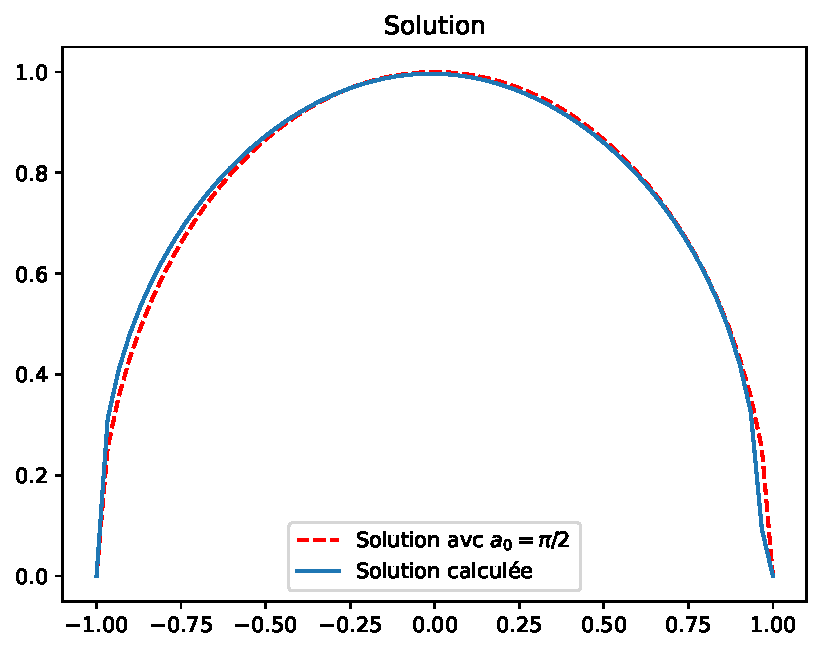
\includegraphics[scale=0.5]{../res/test_sol}
	}
	\subfigure[Évolution des aires]{%
	\label{fig:tst_air}
		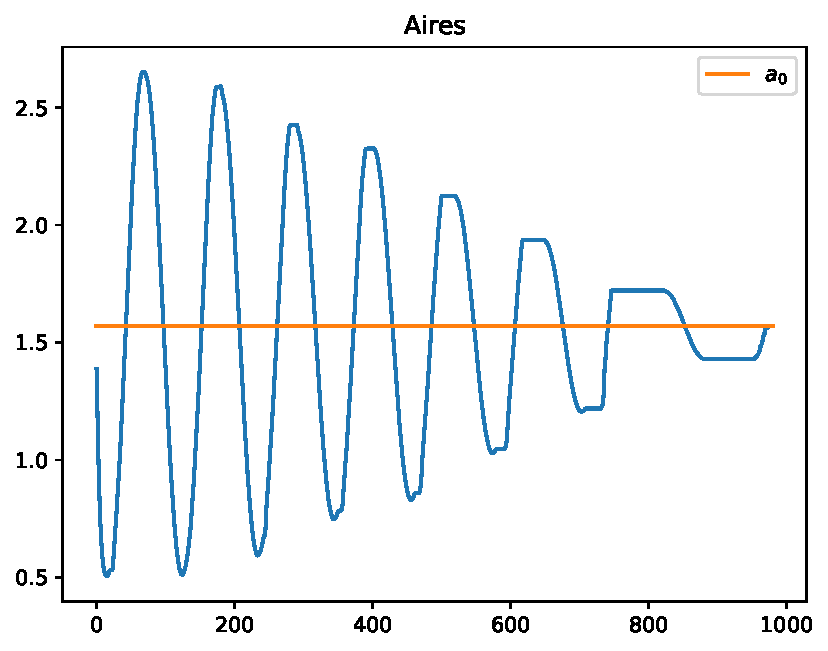
\includegraphics[scale=0.5]{../res/test_aires}
	}
	\subfigure[Évolution des longueurs]{%
		\label{fig:tst_lon}
		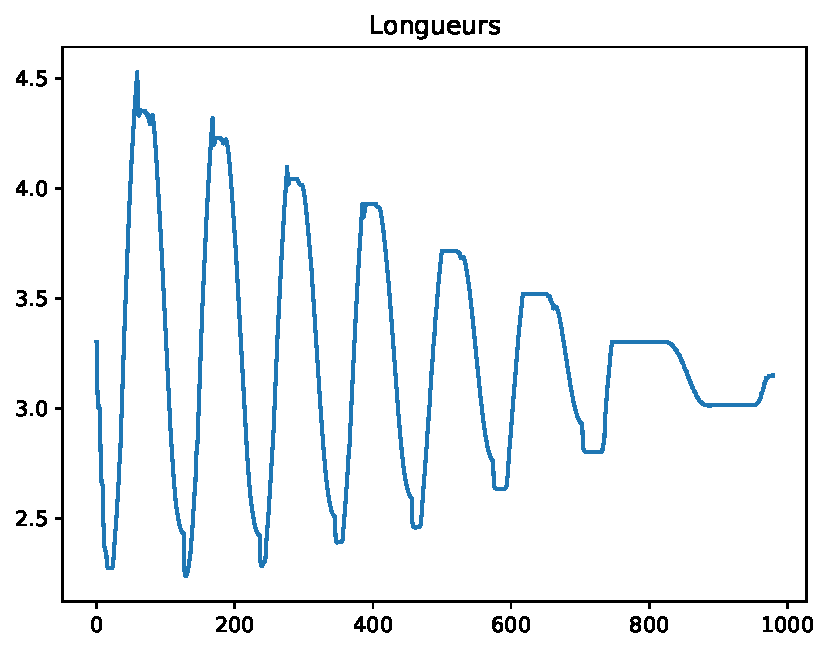
\includegraphics[scale=0.5]{../res/test_longueurs}
	}
	\subfigure[Évolution du Lagrangien]{%
		\label{fig:tst_lag}
		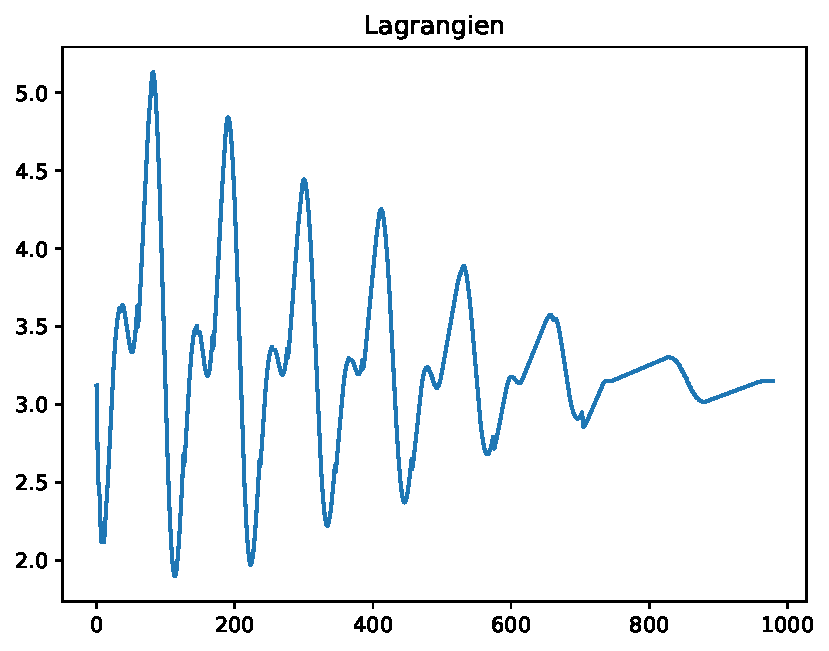
\includegraphics[scale=0.5]{../res/test_lagrangien}
	}
	\caption{Résultats avec $a_0=\frac{\pi}{2}$}
\end{figure}

On a représenté en figure \ref{fig:tst_air}, l'évolution de l'aire de la solution calculée au cours des différentes boucles de l'algorithme. L'évolution de la longueur et du Lagrangien ont aussi été tracées. On peut ainsi visualiser le comportement de l'algorithme : si on est en dessous on va avoir tendence à remonter et inversement. Les boucles des algorithmes \ref{algo:primale} et \ref{algo:duale} permettent d'être sûr d'aller dans le bon sens. Ici, la solution a convergé, c'est-à-dire que l'on a atteint le critère d'arrêt, en 980 itérations de la boucle d'Uzawa. À la fin, on a obtenu un aire valant 1.570357412122347 (très proche de $a_0=\frac{\pi}{2}$), et un périmètre final valant 3.1490304292815354 (on aurait dû trouver $\pi$).


On peut ensuite regarder à quoi ressemblerait la courbe obtenue en prenant une valeur de $a_0$ différente de $\frac{\pi}{2}$. Regardons dans un premier temps en prenant $a_0=1$. Cette fois, l'algorithme converge en 287 itéraions (en 5.6 secondes), et on trouve un périmètre final valant 2.625. La solution est tracée en figure \ref{fig:1}.

De même, la solution obtenue avec $a_0=3$ est tracée en figure \ref{fig:3}. Cette fois-ci, l'algorithme a mis 2\,768 itérations avant de se stopper, et le résulats du périmètre final est 4.622. De manière générale, pour $a_0\geqslant\frac{\pi}{2}$, le nombre d'itéraions est beaucoup plus élevé. Par exemple, en prenant $a_0=4$, l'algorithme a atteint le nombre maximal d'itérations valant $2\cdot10^{5}$ avant de converger.



\begin{figure}
	\centering
	\subfigure[$a_0=1$]{%
		\label{fig:1}
		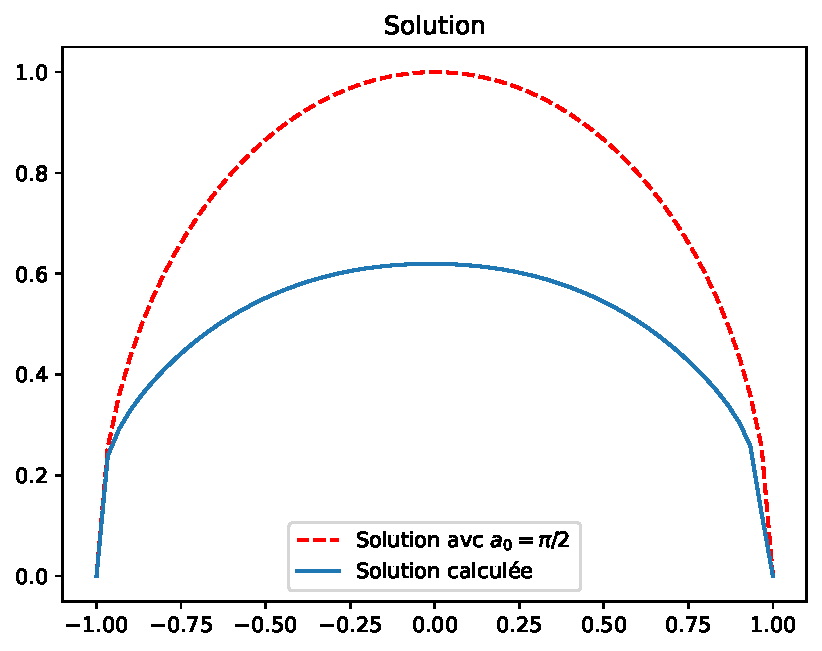
\includegraphics[scale=0.5]{../res/petit_sol}
	}
	\subfigure[$a=3$]{%
		\label{fig:3}
		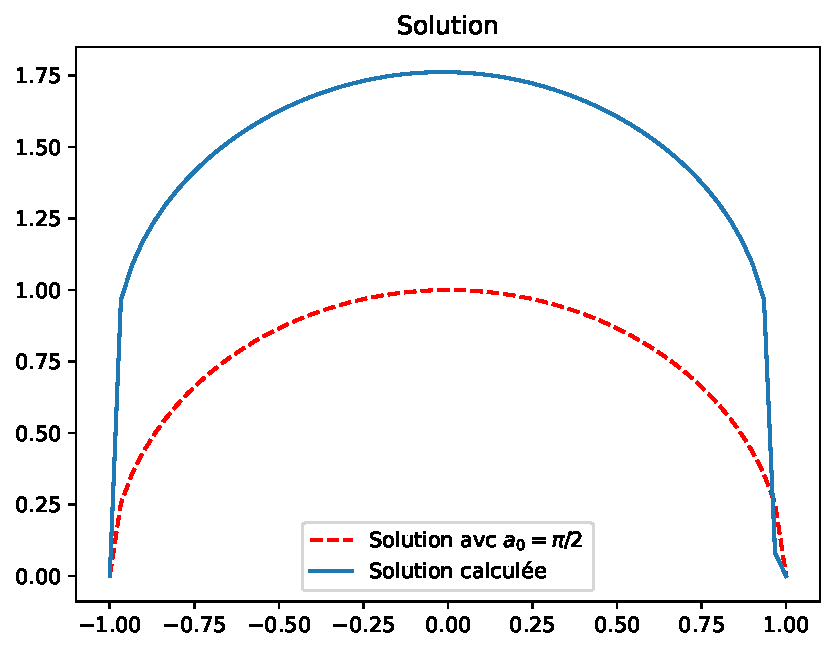
\includegraphics[scale=0.5]{../res/trois_sol}
	}
	\caption{Résultats pour différentes valeurs de $a_0$}
	\label{fig:diff}
\end{figure}






\subsection{D'autres méthodes pour résoudre le problème}

Nous allons dans un premier temps nous intéresser au Lagrangien augmenté \cite{cohen00}. Il s'agit ici de prendre une autre fonction pour le Lagrangien, le \emph{Lagrangien augmenté} :

\begin{eqnarray*}
L_b(f,\lambda)&=& lg(f) + \lambda\left(A(f)-a_0 + c\right) + \frac{b}{2}\left(A(f)-a_0+c\right)^2
\end{eqnarray*}

L'algorithme de résolution reste le même que précédemment, la seule différence est la mise à jour du multiplicateur $\lambda$ : au lieu de rechercher le pas de sorte qu'on ait bien une remontée comme ci-dessus, on applique simplement la formule $\lambda^{n+1} = \lambda^n+b(A(f_k)-a_0)$, où $f_k$ est la solution du problème sans contrainte. La méthode que nous avons essayé d'implémenter n'a pas fonctionné pour le moment.

On peut aussi imaginer d'autre méthodes pour obtenir une solution à ce problème, comme par exemple une méthode de pénalisation.


\bibliographystyle{unsrt-fr}
\bibliography{ref}
\addcontentsline{toc}{section}{Références}




\end{document}